\documentclass[11pt]{article}
\usepackage{acl2014}
\usepackage{times}
\usepackage{url}
\usepackage{latexsym}
\usepackage{graphicx}
\usepackage{floatrow}

\newfloatcommand{capbtabboxsmall}{table}[][6cm]
\newfloatcommand{capbtabboxsmaller}{table}[][3cm]

%\setlength\titlebox{5cm}

% You can expand the titlebox if you need extra space
% to show all the authors. Please do not make the titlebox
% smaller than 5cm (the original size); we will check this
% in the camera-ready version and ask you to change it back.


\title{Heterogeneous Supervisory Data Sources for Semantic Parsing}

\author{First Author \\
  Affiliation / Address line 1 \\
  Affiliation / Address line 2 \\
  Affiliation / Address line 3 \\
  {\tt email@domain} \\\And
  Second Author \\
  Affiliation / Address line 1 \\
  Affiliation / Address line 2 \\
  Affiliation / Address line 3 \\
  {\tt email@domain} \\}

\date{}

\begin{document}
\maketitle
\begin{abstract}
This work presents a preliminary exploration of the opportunities and challenges of learning semantic parsers from heterogeneous semantic annotation sources.
\end{abstract}

\section{Introduction}
Multiple annotated resources capture semantic information, for example FrameNet \cite{framenet}, PropBank \cite{propbank}, VerbNet \cite{vnet}. Each of them the result of pain-staking annotation efforts by teams of linguistics over several years. However, they are the result of largely independent annotation efforts which different make theoretical commitments. In this essay, we consider how we might best leverage such heterogenous resources to improve semantic parsing, so as to let semantic resources created at considerable cost not go to waste.

Systems for semantic parsing tasks have mostly focused on using only a single resource. For instance, Semafor \cite{semafor} is a frame-semantic parsing system based on supervised learning that uses FrameNet data to train a model. The Illinois-semantic role labeling system \cite{illinoisSRL} uses PropBank annotations. Often, a single resource despite being very high quality does not contain comprehensive annotations for every semantic entity and will not cover all semantic concepts. For instance, PropBank annotations are very rich in verbs, but very sparse in nouns. These resources also differ in the granularity of the annotated data - FrameNet frames are semantically finer-grained as compared to the PropBank rolesets. However, together these complementary sources provide a very good and diverse coverage of the semantic space - a fact that should be exploited by systems in order to achieve a better performance on semantic analysis. Preliminary work in dependency parsing has demonstrated that divergent treebanks can be leveraged to improve parsing quality \cite{zhou:2013}.

From a supervised learning perspective, the problem of combining the knowledge across these resources can be viewed as a joint learning problem. If we treat the annotation schema of each resource as one label-space, then we can formulate this as a multitask learning problem across tasks with different label spaces. The goal of a system should then be to learn a model over the different label spaces. This problem also manifests in the information extraction community, where there are multiple knowledge-bases confirming to different ontologies.  

To see an example illustrating the need for models that integrate resources, consider the following sentence:
\begin{quote}
\textit{The award \texttt{celebrates} businesses that \texttt{innovate} products which \texttt{appeal} to social good.}
\end{quote}

The three predicates in the above sentence have been rendered in a different font. The frame-semantic parsing output from Semafor is shown in Figure \ref{fig:semaforOutput}. While the system completely misses two of the predicates, one of them \texttt{appeal} is not recognized correctly. The reasons for the errors are: the first two predicates do not have an annotation in FN, and the third one is annotated in the context of appeals in a court of law. More importantly, all three predicates have an appropriate annotation in PB.

\begin{figure*}
\caption{Frame semantic parsing output from Semafor for an example sentence.}
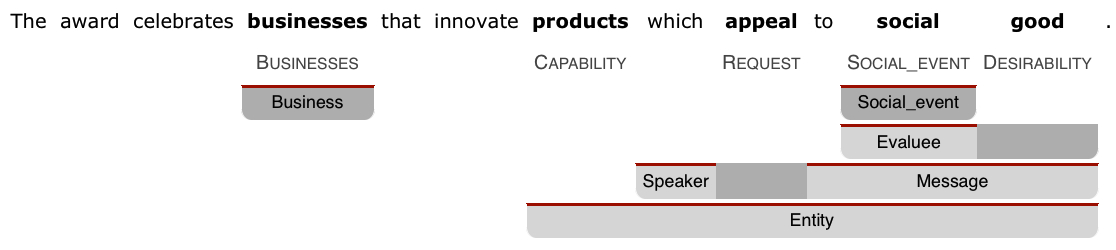
\includegraphics[scale=0.4]{semafor_output.jpg}
\label{fig:semaforOutput}
\end{figure*}


The following list indicates the scenarios where a joint model based on both FrameNet and PropBank data can improve frame-semantic parsing accuracies in a system like Semafor. The examples and numbers presented below were obtained from the latest FrameNet release (1.5) and for PB we consider only the WSJ section of the annotations.
\begin{itemize}
\item Frames with none or very few annotations in FN. The frame \textit{Manipulation} does not have any annotations for the verb \texttt{hold}, whereas PB-WSJ has 117 instances (that had an extractable argument mapping) for this frame-target combination. The frame \textit{Experiencer\_obj} has several predicates without any annotations, for example \texttt{appeal}, \texttt{harass}, \texttt{worry}, \texttt{boggle}. The first three of these have annotations in the PB-WSJ data. There are 984 such predicates in FN that have been assigned to frames, but with no sentence annotations available.
\item Frames with few known targets or targets with no associated frames. For example, the frame \textit{Giving} has 19 known verbs as targets in FN. Synonyms of \textit{giving} such as \texttt{allot}, \texttt{assign}, \texttt{designate}, \texttt{allocate} are not present in FN. Overall, there are 475 verbs in the PB WSJ data that are not targets for any frame in FrameNet. Some examples are: \texttt{involve}, \texttt{lurk}, \texttt{nominate}, \texttt{ladle}, \texttt{entice}, \texttt{bank}.
\end{itemize}
Ideally, a joint learning system should also be able to suggest new targets for a frame based on the lexical similarity with the frame's existing targets.

Linguistic resources to map the different annotations have been built, but to a very limited extent. SemLink \cite{semlink} is one such database that maps and unifies different lexical resources of semantic information: such as PropBank (PB), FrameNet (FN), VerbNet (VN). The mappings that SemLink provides are available at two different levels: (a) sentence level parallel annotations - the WSJ section of the PB data has been annotated with the appropriate frames and frame-elements as well as VerbNet classes wherever possible, thereby giving detailed PB, VN and FN annotations for each sentence (b) concept/roleset level mappings - these are coarse-level mappings defined between a PB roleset and a VN roleset or a FN frame and a VN roleset. These mappings can be one-to-one, one-to-many or many-to-many depending on the semantic generality of the involved rolesets. To go from a PB roleset to a FN frame, one has to go via the VN roleset first.

In this work, we will focus on Semafor as the target system whose performance we want to improve. We are hence interested in using the SemLink mappings to get FN compatible data. The type (a) mappings can be directly used to augment the FN annotations; in the next section we present an analysis on the quantity and usability of the available mappings. Using the type (b) annotations first requires disambiguating the frame-to-roleset labels and then aligning the predicate arguments of the roleset with those expected in the frame. Note that the two argument sets might be of different cardinality.

\section{Data analysis}
We present some statistics of the data resources in Tables \ref{tab:wsjstats} and \ref{tab:annoUnit}. The first table summarizes the SemLink mappings for the PB WSJ data. The total number of annotated PB instances are 74977, a majority of which do not have the corresponding FN labels due to various difficulties in mapping them. Around 31\% of the predicates have the frame label \textit{IN} meaning ``indefinite''. For these cases the mapping from VN to FN does not clearly indicate which Frame the instance should be. About 20\% of the instances are labeled \textit{NF} or ``no frame'' as FrameNet currently does not have an appropriate frame class for the semantic concept represented by the PB predicate. Of the remaining, 21\% are incomplete as they only have frame labels and no argument annotations. Most of these are predicates with modifier arguments. This leaves about 29\% usable mappings, 9\% of which had argument pointer and other issues. Eventually, we were able to extract about 15323 instances.

The second table compares the extracted PB-WSJ annotations with the original FN annotations (version 1.4) used to train the Semafor model. The number of annotations at the sentence-level and frame-level are shown. It is evident that FN has a much higher annotation density - around 9 frames per sentence, as compared to around 1.2 for the PB derived data .


\begin{table}
\caption{Statistics of PB-WSJ data from SemLink}
\label{tab:wsjstats}
\begin{tabular}{|l|c|c|} \hline
FN frame annotation & Verb tokens & \% of all \\
& from PB & \\ \hline \hline
Frame label = \textit{NF} & 14624 & 20\%\\ \hline
Frame label = \textit{IN} & 22982 & 31\% \\ \hline
Frame with no & 15533 & 21\% \\ 
arguments  & & \\\hline
Frame with at least & 15323 & 20\% \\ 
1 argument mappable & & \\ \hline
Instances not mapped & 6516 & 9\% \\ 
due to other issues & & \\ \hline \hline
Total PB predicate & 74977 & 100\% \\
tokens (instances) & & \\ \hline
\end{tabular}
\end{table}

\begin{table}
\caption{Comparison of annotation density}
\begin{tabular}{|l|c|} \hline
\label{tab:annoUnit}
Annotation unit & Count \\\hline \hline
Sentences in FN 1.4 & 2780 \\ 
Annotation sets in FN 1.4 & 23940 \\ % new framenet: 27409
(i.e frame instances) & \\ 
Annotation density & 8.6 \\ \hline \hline
Sentences in PB WSJ data &  38594 \\ 
Verb tokens in PB WSJ & 74977 \\ 
Annotation density &  1.9 \\\hline \hline
Sentences extracted & 12896 \\ 
from SemLink PB-WSJ & \\ 
Annotation sets extracted & 15323\\ 
Annotation density & 1.2 \\ \hline 
\end{tabular}
\end{table}



The mappings we obtained increase the number of annotations for around 170 frames. Figure \ref{fig:framesBarchart} shows a stacked bar-chart plotting the annotations for every frame, sorted in decreasing order of additional frames obtained. The highest is around 1500 new annotations for the frame \textit{Statement}.
\begin{figure*}
\caption{The number of new annotations per frame obtained upon extracting the WSJ mapping from SemLink. The bars are coloured (red) to indicate the contribution from the new annotations. Only frames for which new annotations were found are shown.}
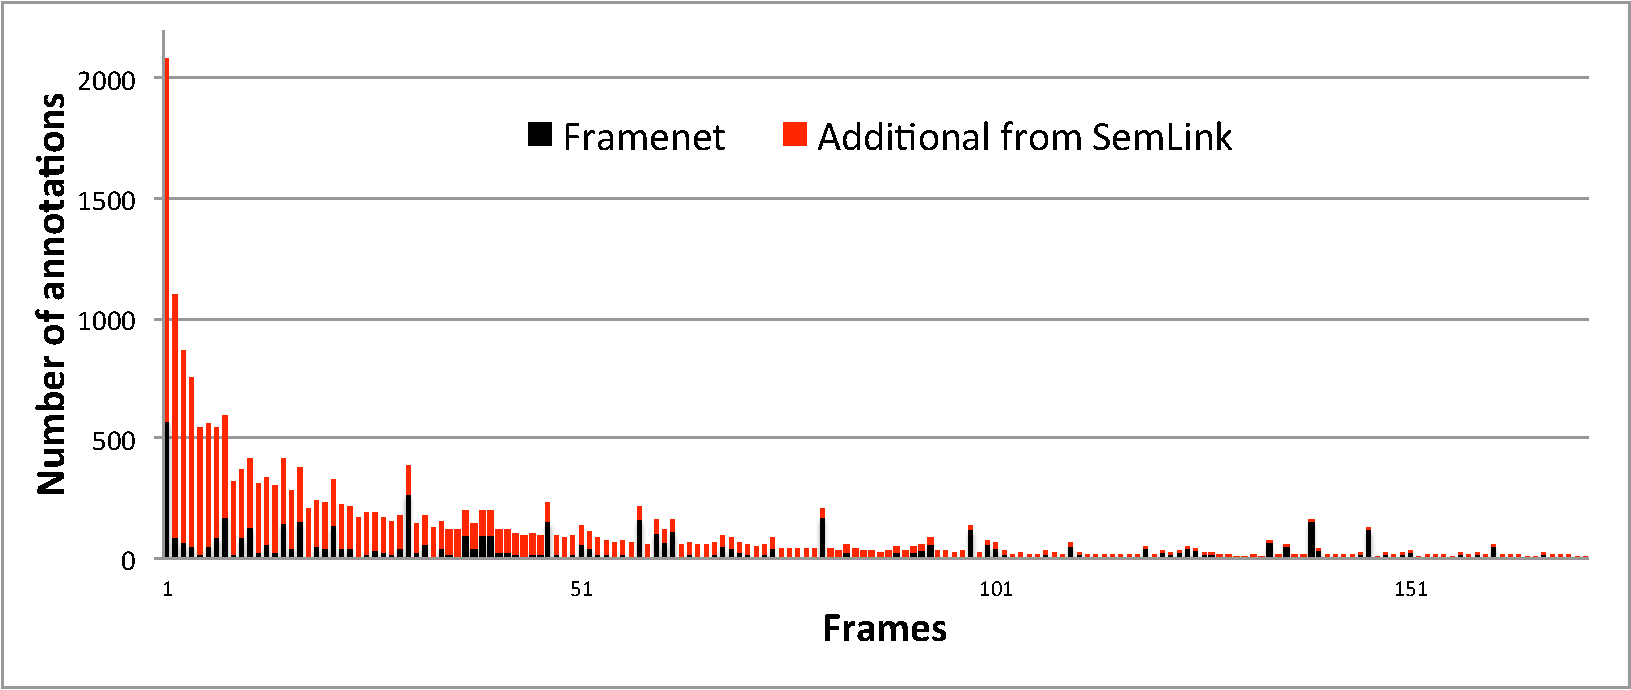
\includegraphics[scale=0.5]{framesBarchart.pdf}
\label{fig:framesBarchart}
\end{figure*}

\subsection{Noisy SemLink annotations}
Since SemLink was built, FrameNet has updated frame definitions, some new frames were introduced and old ones deleted or divided into finer categories, irrelevant predicates moved to proper frames etc. Hence some of the SemLink annotations are obsolete and sub-optimal. For example, the frame \textit{Statement} does not contain the target \texttt{complain.v} anymore as a new frame \textit{Complain} was introduced. There are around 3000 such instances with obsolete annotations. These can be detected easily and they are also not semantically absurd, but correcting these will require re-annotation on a case-by-case basis.

Additionally, there are some mistakes in some of the annotations due to the existence of multiple frame matches for a particular predicate. For example, in the sentence \textit{McMoRan Energy Partners will be \texttt{liquidated}}, the frame for \texttt{liquidate} is \textit{Killing} - all 14 occurrences of liquidate have this error. The sentence \textit{Speaker Jim Wright.. attempting to \texttt{direct} the president} has the frame annotation \textit{Behind\_the\_scenes} which refers to film ``direction''. There are 17 instances with this frame erroneously marked. These kind of errors are hard to detect.

\section{Evaluation}
As indicated in the introduction, a model encompassing multiple resources can fill in various types of gaps in the FN annotations. It is infeasible to measure improvements for predicates which are not already frame targets in FN. For existing frame-predicates with no argument annotations, the SemLink mappings can be used as test data.

\section*{Acknowledgments}

% include your own bib file like this:
\bibliographystyle{acl}
\bibliography{refs}

\end{document}
